\documentclass{article}

% if you need to pass options to natbib, use, e.g.:
%     \PassOptionsToPackage{numbers, compress}{natbib}
% before loading neurips_2026

% The authors should use one of these tracks.
% Before accepting by the NeurIPS conference, select one of the options below.
% 0. "default" for submission
\usepackage{neurips_2026}
% the "default" option is equal to the "main" option, which is used for the Main Track with double-blind reviewing.
% 1. "main" option is used for the Main Track
%  \usepackage[main]{neurips_2026}
% 2. "position" option is used for the Position Paper Track
%  \usepackage[position]{neurips_2026}
% 3. "eandd" option is used for the Evaluations & Datasets Track
 % \usepackage[eandd]{neurips_2026}
% 4. "creativeai" option is used for the Creative AI Track
%  \usepackage[creativeai]{neurips_2026}
% 5. "sglblindworkshop" option is used for the Workshop with single-blind reviewing
 % \usepackage[sglblindworkshop]{neurips_2026}
% 6. "dblblindworkshop" option is used for the Workshop with double-blind reviewing
%  \usepackage[dblblindworkshop]{neurips_2026}
% 7. "education" option is used for the Education Track
%  \usepackage[education]{neurips_2026}


% After being accepted, the authors should add "final" behind the track to compile a camera-ready version.
% 1. Main Track
 % \usepackage[main, final]{neurips_2026}
% 2. Position Paper Track
%  \usepackage[position, final]{neurips_2026}
% 3. Evaluations & Datasets Track
 % \usepackage[eandd, final]{neurips_2026}
% 4. Creative AI Track
%  \usepackage[creativeai, final]{neurips_2026}
% 5. Workshop with single-blind reviewing
%  \usepackage[sglblindworkshop, final]{neurips_2026}
% 6. Workshop with double-blind reviewing
%  \usepackage[dblblindworkshop, final]{neurips_2026}
% Note. For the workshop paper template, both \title{} and \workshoptitle{} are required, with the former indicating the paper title shown in the title and the latter indicating the workshop title displayed in the footnote.
% For workshops (5., 6.), the authors should add the name of the workshop, "\workshoptitle" command is used to set the workshop title.
% \workshoptitle{WORKSHOP TITLE}
% 7. Education Track
% \usepackage[education, final]{neurips_2026}

% "preprint" option is used for arXiv or other preprint submissions
 % \usepackage[preprint]{neurips_2026}

% to avoid loading the natbib package, add option nonatbib:
%    \usepackage[nonatbib]{neurips_2026}

\usepackage[utf8]{inputenc} % allow utf-8 input
\usepackage[T1]{fontenc}    % use 8-bit T1 fonts
\usepackage{hyperref}       % hyperlinks
\usepackage{url}            % simple URL typesetting
\usepackage{booktabs}       % professional-quality tables
\usepackage{amsfonts}       % blackboard math symbols
\usepackage{nicefrac}       % compact symbols for 1/2, etc.
\usepackage{microtype}      % microtypography
\usepackage{xcolor}         % colors
\usepackage{amsmath}
\usepackage{amssymb}
\usepackage{graphicx}
\usepackage{float}
\usepackage{placeins}

\newcommand{\pct}{\%}

% Note. For the workshop paper template, both \title{} and \workshoptitle{} are required, with the former indicating the paper title shown in the title and the latter indicating the workshop title displayed in the footnote. 
\title{Controllability Across Composition, Topology, and Function in Language-Model Protein Generation}


% The \author macro works with any number of authors. There are two commands
% used to separate the names and addresses of multiple authors: \And and \AND.
%
% Using \And between authors leaves it to LaTeX to determine where to break the
% lines. Using \AND forces a line break at that point. So, if LaTeX puts 3 of 4
% authors names on the first line, and the last on the second line, try using
% \AND instead of \And before the third author name.


\author{%
  David S.~Hippocampus\thanks{Use footnote for providing further information
    about author (webpage, alternative address)---\emph{not} for acknowledging
    funding agencies.} \\
  Department of Computer Science\\
  Cranberry-Lemon University\\
  Pittsburgh, PA 15213 \\
  \texttt{hippo@cs.cranberry-lemon.edu} \\
  % examples of more authors
  % \And
  % Coauthor \\
  % Affiliation \\
  % Address \\
  % \texttt{email} \\
  % \AND
  % Coauthor \\
  % Affiliation \\
  % Address \\
  % \texttt{email} \\
  % \And
  % Coauthor \\
  % Affiliation \\
  % Address \\
  % \texttt{email} \\
  % \And
  % Coauthor \\
  % Affiliation \\
  % Address \\
  % \texttt{email} \\
}


\begin{document}


\maketitle


\begin{abstract}
Protein language models generate plausible sequences, but reliably directing them toward multi-objective, user-specified properties remains difficult. We ask whether instruction tuning can give a general-purpose language model such control without training a protein model from scratch. We present Aria, a feature-conditioned protein generator that instruction-tunes
Llama-3.1-8B-Instruct on nearly 349k Swiss-Prot proteins, each described by a
partial, randomly sampled subset of up to thirteen biophysical, structural and functional descriptors expressed directly in the prompt. On a leakage-controlled held-out set of 35,115 proteins, separated from training by MMseqs2 clustering, instruction tuning improves adherence on every recomputable axis: length within ±10\pct increases from 11.6\pct to 88.8\pct, hydrophobicity from 62.4\pct to 86.9\pct, stability from 52.9\pct to 72.2\pct, and exact cysteine-count adherence from 23.3\pct to 68.9\pct. Topological control improves similarly, with transmembrane-helix MCC increasing from 0.28 to 0.87 and signal-peptide MCC from 0.07 to 0.74. Exact Pfam-domain recovery improves over the base model but remains low overall at 2.9\pct and is strongly associated with domain exposure during training. Scoring each generation against a different held-out specification reduces adherence on every recomputable axis, by up to 77 percentage points, so what the benchmark measures is response to the prompt rather than common property values. Additionally, we demonstrate that adding up to twelve additional descriptors does not reduce adherence to a fixed length target, indicating that control was not limited simply by prompt load. We then show that adherence evaluators could guide further improvement after supervised instruction-tuning. In PF00416 (ribosomal protein uS13), one natural-sequence-anchored round of direct preference optimization (DPO)  \citep{rafailov2023dpo} increased mean ESMFold pLDDT from 49.4 to 57.6, still short of the 78.0 mean of natural family members. These results show that instruction tuning can repurpose a general language model for property-conditioned protein generation, while evaluator-guided preference optimization offers a route to further improve an existing generator cost-effectively.
\end{abstract}



\section{Introduction}


\begin{figure}[t]
  \centering
  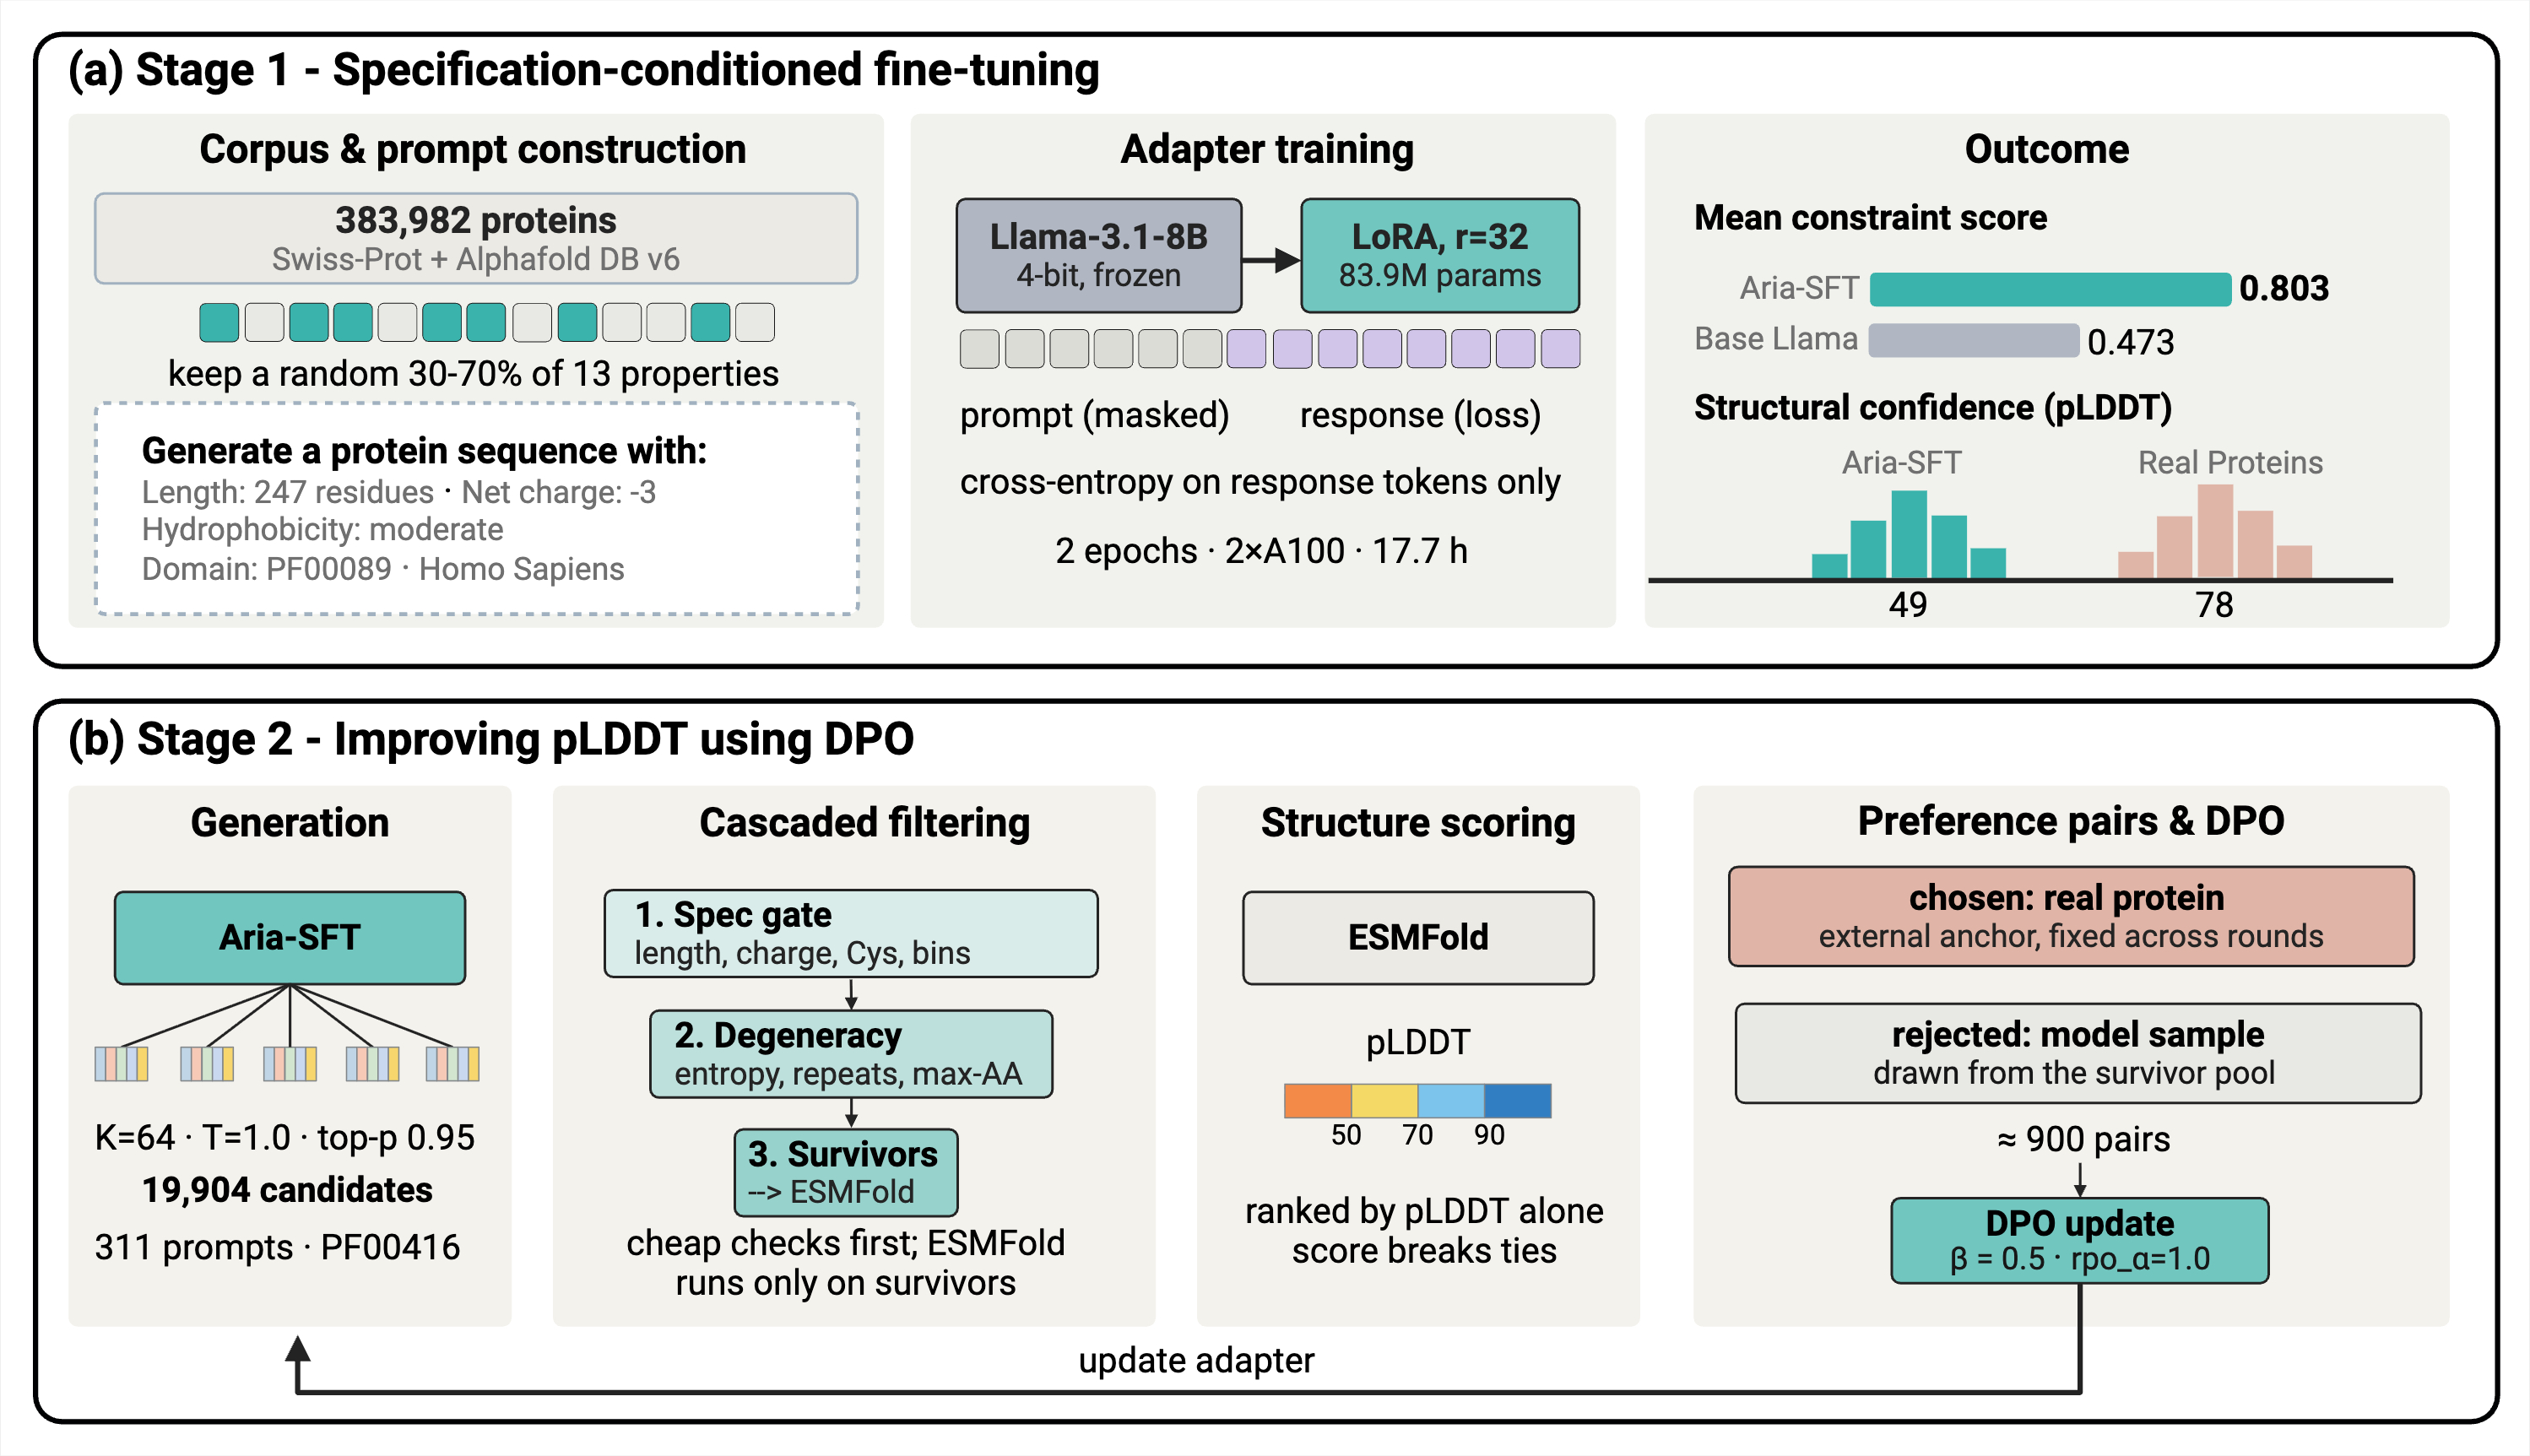
\includegraphics[width=\linewidth]{figures/Fig1_V2.jpeg}
  \caption{The Aria training and preference-optimization workflow.
  (a) During specification-conditioned fine-tuning, each example pairs
  a specification containing a randomly selected 30--70\pct{} subset of thirteen
  protein descriptors with its natural sequence; loss is computed only over the
  sequence. (b) For ribosomal protein uS13, generated candidates are
  evaluated using the specification gate and sequence filters before structural
  prediction with ESMFold. Natural sequences provide preferred responses for DPO,
  anchoring optimization to specification-consistent family members while
  increasing predicted structural confidence. Together, these stages illustrate
  how the same measurements used to evaluate adherence can also provide
  post-training feedback.}
  \label{fig:pipeline}
\end{figure}
Protein language models have made sequence generation routine. Autoregressive
models trained on large sequence corpora, among them ProGen
\citep{madani2023progen}, ProGen2 \citep{nijkamp2023progen2} and ProtGPT2
\citep{ferruz2022protgpt2}, emit sequences that fold and resemble natural
proteins, and encoder families such as ESM \citep{lin2023esm2} represent them
well enough to support structure prediction. Producing a plausible protein is no
longer the difficulty. Directing that production is.

Two obstacles stand in the way, and they compound each other. The first is that the interface is often narrow. For example, 
ProGen and ProGen2 condition on family or keyword tags, ProtGPT2 does not
condition at all, and ProLLaMA \citep{lv2026prollama} exposes a single
categorical axis, the protein superfamily, treating physicochemical properties
as a decode-time filter rather than as targets a user may set. Work that does address attributes directly steers through learned tokens or model-internal interventions \citep{ismail2025cbplm, luo2026prefixprot, liu2025ctrlprot, hayes2025esm3}, or aligns free-text function descriptions with sequence \citep{liu2025proteindt, wang2024instructprotein}, rather than accepting a user-provided textual specification. The second obstacle is measurement. Evaluations across recent protein-generation studies \citep{madani2023progen,nijkamp2023progen2,
ferruz2022protgpt2} are dominated by perplexity, predicted structural confidence \citep{jumper2021alphafold}, and template-modeling scores \citep{zhang2004tmscore}. These metrics ask whether a generation resembles a protein, not whether it carries the properties that were requested. This distinction matters in practice: a model that disregards a stated net charge while emitting a well-folded sequence scores well on commonly used measures, and the failure surfaces only downstream, during purification or formulation.
Instruction tuning \citep{zhang2023instructiontuning} addresses both at once. A
general instruction-tuned model already accepts conditions stated in natural
language, so a conjunctive, partial request needs no bespoke interface, only
training data in which such requests appear; and for many properties the request
is verifiable, since the property can be recomputed on the generated sequence
with the function that wrote the specification.
Using this approach, we instruction-tune Llama-3.1-8B-Instruct \citep{dubey2024llama3} with QLoRA \citep{dettmers2023qlora,hu2022lora} on nearly 349k Swiss-Prot proteins, each
described by a partial, randomly sampled subset of thirteen physicochemical, developability, topological, and functional descriptors written into the prompt, and evaluate on
35{,}115 held-out specifications separated from training at the level of
sequence clusters. Adherence improves on every axis we can recompute, after a single low-rank run requiring approximately 35 GPU-hours and updating
only 1\pct{} of the parameters, without protein-specific pre-training.
Composition transfers well (hydrophobicity 62.4\pct{} to 86.9\pct, exact cysteine
count 23.3\pct{} to 68.9\pct, length within $\pm$10\pct{} 11.6\pct{} to
88.8\pct) and so does topology (transmembrane helix, Matthews correlation 0.275
to 0.869; signal peptide, 0.073 to 0.739). Functional control remains more difficult: exact Pfam-domain recovery is 2.9\pct{} overall, but success increases strongly with domain exposure during training. Because these evaluations are sequence-based, they can serve not only as scores but also as training signals. We therefore apply one round of direct preference optimization (DPO) to PF00416, the ribosomal protein uS13 family, using the natural sequence as the preferred response. This tests whether predicted structural confidence can be improved without sacrificing adherence. Mean ESMFold pLDDT increases from 49.4 to 57.6, while both property-gate and sequence-filter pass rates also increase. 

Together, these results show that a general instruction-tuned model can be repurposed into a property-conditioned protein generator through a single parameter-efficient fine-tuning run with no prior protein training, improving measurable adherence rather than
protein plausibility alone. They further show that the same evaluations used to
verify adherence can guide targeted improvements after supervised fine-tuning.
Although demonstrated here for a general-use language model, this formulation provides a testable route to improving adherence in existing protein language models.

\section{Results}

\begin{figure}[b!]
\centering
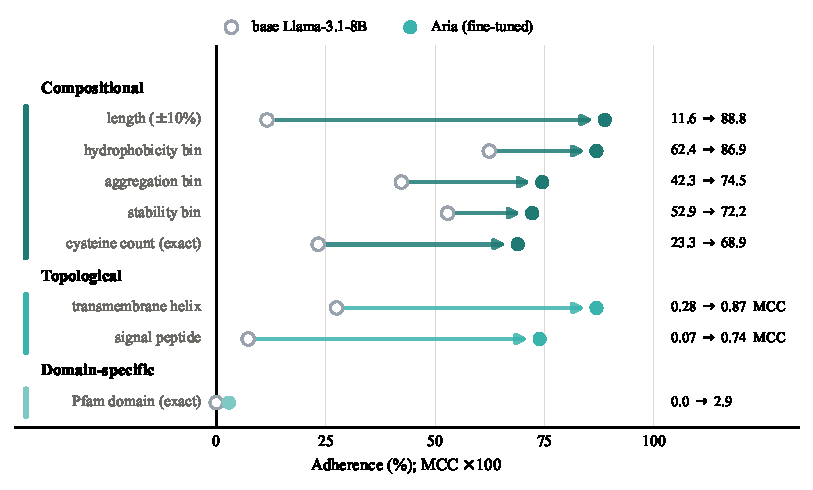
\includegraphics[width=\linewidth]{figures/fig-tiers.pdf}
\caption{The controllability hierarchy. Each row is one scored property: left
marker the base model, right marker Aria, the line between them what
fine-tuning bought. Rows are read independently, so percentage and MCC rows
share one axis with MCC $\times$100. Enzyme class is omitted because
its measurement is confounded (Appendix~\ref{app:ec}).}
\label{fig:tiers}
\end{figure}

Instruction-tuning improves all measured properties, but the magnitude of control follows a clear hierarchy (Figure~\ref{fig:tiers}, Table~\ref{tab:controls}). Properties determined by overall composition or recognizable topological signals are strongly controllable, whereas exact domain identity remains difficult. We organize the results around this distinction.
\paragraph{Tier 1: Composition and Developability.}
Fine-tuning first teaches the model to return the requested output format: the fraction of generations containing a bare sequence rather than prose rises from 0\pct{} to 99.9\pct. Beyond formatting, adherence improves across every measured sequence-derived property. Length adherence rises from 11.6 to 88.8\pct, hydrophobicity from 62.4 to 86.9\pct, and exact cysteine-count adherence from 23.3 to 68.9\pct; aggregation and stability show similar gains (Figure~\ref{fig:tiers}).
While exact numerical control remains less precise for charge, the correlation between requested and realized net charge rises from $r=0.26$ to $r=0.89$, showing that the model responds strongly to the requested direction (Table~\ref{tab:controls}, Appendix~\ref{app:charge}). 

\paragraph{Tier 2: Topology.} Transmembrane-helix recall rises from 14.0 to
86.5\pct{} and MCC from 0.275 to 0.869; signal peptides from 6.6 to 61.4\pct{}
and 0.073 to 0.739. Positive-class precision stays high (91.4\pct{} and 93.2\pct), so
recall is not bought by inserting hydrophobic stretches indiscriminately.
%Topological features have diffuse but characteristic signatures, and the model acquires them as readily as Tier 1 by distributed regularities, not exact residue placement. 

\paragraph{Tier 3: Domain Identity.}
Domains are assigned with \texttt{hmmscan} against Pfam-A, where lower $E$-values indicate stronger sequence-profile matches. At the default reporting threshold, the requested domain is detected in 2.90\% of fine-tuned generations (520 of 17{,}941), compared with none of 15{,}140 base-model generations. The few highly significant assignments are nevertheless specific: among the 145 generations receiving any match at $E\leq10^{-10}$, 71.0\% match the requested domain. The aggregate recovery rate is partly depressed by uneven training exposure: many requested domains are absent or rare in training, and success increases markedly with their representation (Appendix~\ref{app:domain}, Figure \ref{fig:domain}). Thus, the model learns targeted signatures for some represented domains but does not provide reliable exact-domain control.


\subsection{Adherence reflects prompt conditioning}

Raw adherence can be inflated by common property values, even if a model ignores
the prompt. We therefore compare Aria with two request-blind controls: a constant
baseline that always predicts the most frequent training value, and a mismatch
control that scores each generated sequence against a different held-out
specification. Aria exceeds both controls on all six sequence-derived properties
(Table~\ref{tab:controls}); mismatching the specifications reduces mean adherence by between 20.3 points on net charge and 76.9 points on length. Compositional adherence also remains similar when the requested Pfam
family is absent from training (71.4\%, compared with 71.0\% for represented
families). The measured control therefore reflects response to the specification
rather than common corpus values or memorization of protein families.

\subsection{Additional constraints do not weaken length control}

We next test whether control deteriorates as more properties are included in the same specification. For each of 200 held-out proteins, we construct thirteen prompts with an identical length target while adding one further property at each step. Length adherence remains between 84 and 92\%, with no significant trend as constraints are added (slope $+0.028$, 95\% CI $[-0.006,+0.061]$; Appendix~\ref{app:ladder}). The probability of satisfying all requested sequence-derived properties decreases as their number grows, but the observed decline is consistent with multiplying their individual success probabilities. Thus, adding constraints does not measurably weaken length control; the lower joint-pass rate primarily reflects the arithmetic difficulty of satisfying more conditions simultaneously.


\subsection{Anchored DPO improves adherence and predicted structural confidence}
\begin{table}[b]
\caption{Prompt-conditioned adherence on directly recomputable properties.
The value of $n$ is the number of valid Aria generations whose specification
requested the corresponding property. Bracketed values are 95\% Wilson
confidence intervals for Aria's adherence rate. Aria is compared with the
constant and prompt-mismatch controls described in
Appendix~\ref{app:method}.}
\label{tab:controls}
\centering
\small
\begin{tabular}{lrrrr}
\toprule
Property
    & $n$
    & \textbf{Aria [95\% CI]}
    & Constant
    & Mismatch \\
\midrule
Length ($\pm10\pct$)
    & 19{,}140
    & \textbf{88.8\pct{} [88.4, 89.3]}
    & 19.8\pct
    & 11.9\pct \\
Hydrophobicity bin
    & 19{,}030
    & \textbf{86.9\pct{} [86.4, 87.3]}
    & 72.4\pct
    & 52.3\pct \\
Aggregation bin
    & 18{,}966
    & \textbf{74.5\pct{} [73.9, 75.2]}
    & 34.2\pct
    & 33.0\pct \\
Stability bin
    & 18{,}998
    & \textbf{72.2\pct{} [71.5, 72.8]}
    & 55.0\pct
    & 51.7\pct \\
Cysteine count (exact)
    & 18{,}853
    & \textbf{68.9\pct{} [68.3, 69.6]}
    & 17.5\pct
    & 10.4\pct \\
Net charge ($\pm2$)
    & 18{,}919
    & \textbf{35.2\pct{} [34.5, 35.9]}
    & 25.3\pct
    & 14.9\pct \\
\bottomrule
\end{tabular}
\end{table}

We next asked whether the measurements used to evaluate generation could also guide post-training. We studied ribosomal protein uS13 (Pfam PF00416), using 311 natural sequences for training and 260 cluster-separated sequences for held-out evaluation. For each training specification, the SFT model generated 64 candidates. Candidates passing the property gate and sequence filters were evaluated with ESMFold \citep{lin2023esm2}. The natural sequence corresponding to the specification served as the preferred response, and up to three eligible model generations served as rejected responses when their pLDDT was at least five points lower. This procedure yielded 929 preference pairs. Starting from the SFT checkpoint, we performed one DPO-based training stage
\citep{rafailov2023dpo} with an auxiliary negative-log-likelihood term on the
preferred responses, as used in RPO \citep{pang2024rpo}. ESMFold scores determined pair inclusion, whereas training used the resulting preference ordering rather than pLDDT as a differentiable reward.

On 260 matched held-out prompts, one DPO update improves all principal population rates. Mean ESMFold pLDDT rises by 8.2 points, from 49.4 to 57.6 ($p<10^{-11}$), and the fraction reaching pLDDT $\geq70$ rises from 6.9 to 21.9\%. For comparison, the 571 natural PF00416 sequences have a mean ESMFold pLDDT of 78.0 under the same pipeline.  Specification-gate passage increases from 16.9 to 25.8\%, sequence-filter passage from 88.5 to 96.5\%, and passage of both from 16.2 to 25.4\%. The strict composite requiring the gate, filters, and pLDDT threshold rises from 0.4 to 7.3\% (1 to 19 of 260). Generations remain less similar to the training set than natural family members are (Appendix~\ref{app:compute}). Predicted confidence therefore improves without sacrificing specification
adherence or sequence plausibility (Figure~\ref{fig:dpo}).

\begin{figure}[t]
\centering
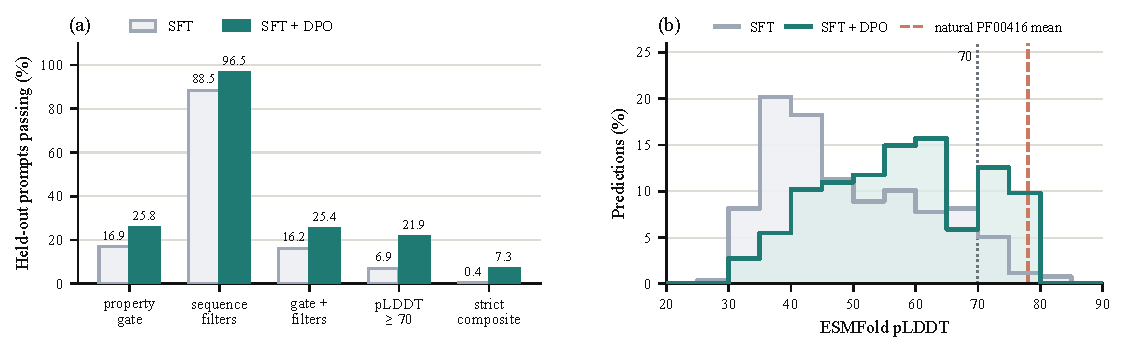
\includegraphics[width=\linewidth]{figures/fig-dpo.pdf}
\caption{One-sample PF00416 evaluation on 260 matched held-out prompts, with
one generation per model per prompt. (a) Pass rates for the
sequence-derived property gate, sequence filters, their conjunction, ESMFold
pLDDT $\geq 70$, and the strict composite requiring all criteria.
(b) ESMFold pLDDT distributions. The dotted line marks the pLDDT
threshold of 70; the dashed line is the mean of 571 natural PF00416 sequences
under ESMFold (78.0).}
\label{fig:dpo}
\end{figure}

\section{Discussion}
Across the tested axes, Aria shows a hierarchy of controllability. Gains are strongest for physicochemical, developability, and topological properties, whereas exact Pfam-domain recovery remains low. Request-blind controls show that the composition gains are not explained solely by an unconditional shift in model outputs. On cluster-separated families, composition control persists, whereas exact domain recovery increases with family exposure (Appendix~\ref{app:domain}). Controllability therefore depends on both the requested property and, for domain identity, training exposure. On PF00416, one natural-sequence-anchored DPO stage raises mean ESMFold pLDDT from 49.4 to 57.6 and improves the property gate, sequence filters, and strict composite under matched one-sample evaluation. Nevertheless, 57.6 remains below the ESMFold mean of 78.0 for the natural PF00416 reference set. Therefore, one round closes 29\% of the distance between the supervised model and natural sequences, so the improvement is substantial yet partial.

Several limitations remain. All results come from a single training run of one 8B model, and behavior at other scales is untested. The baseline is an unadapted general model; a matched comparison measuring the incidental adherence on purpose-built protein language models such as ProLLaMA is our natural next step and is the subject of ongoing work. Additionally, the preference-optimization result rests on a single Pfam family and requires a natural sequence for that family as the preferred response, so it does not apply to a specification for which no natural example exists. 

Within these bounds, the study demonstrates a parameter-efficient route to multi-objective, property-conditioned protein generation. More broadly, the measurement-to-feedback strategy may improve adherence in an existing protein generator whenever the requested property can be reliably evaluated.

\bibliographystyle{plainnat}
\bibliography{references}

\newpage
\appendix
\section{Method}\label{app:method}


Aria is built in two stages (Figure~\ref{fig:pipeline}). 

\textbf{Corpus and specifications.} From the reviewed subset of UniProt
\citep{uniprot2023} we keep sequences of 20--512 residues with canonical
residues, no fragments and no duplicates, leaving $\sim$384k proteins. To
prevent leakage we cluster with MMseqs2 \citep{steinegger2017mmseqs2} at
30\pct{} identity and 80\pct{} coverage and split at the \emph{cluster} level:
348{,}867 training and 35{,}115 held-out proteins, no held-out protein above
30\pct{} identity to any training protein. Thirteen descriptors span four
families (Appendix~\ref{app:desc}): physicochemical and developability
properties computed from the sequence with Biopython \citep{cock2009biopython}
and an AGGRESCAN scale \citep{conchillosole2007aggrescan}; structural and
topological properties from AlphaFold \citep{jumper2021alphafold} and UniProt
annotations; and curator-assigned functional annotations. Each specification
contains a random 30--70\pct{} subset of the descriptors a protein has (3--10
per prompt, mean 6.6), which trains the model for the realistic
under-specified case. The target completion is the bare sequence.

\textbf{Training.} QLoRA \citep{dettmers2023qlora, hu2022lora} on
Llama-3.1-8B-Instruct \citep{dubey2024llama3}: 4-bit base, rank-32 adapter
($\alpha=16$), two epochs, loss on the completion only. 83.9M trainable
parameters, $\sim$35 GPU-hours. No protein-specific pre-training.

\textbf{Evaluation.} Adherence is computed only over specifications that
requested a property, so $n$ varies per property. Six axes are recomputed with
the feature code that built the prompt; applying it to the reference Swiss-Prot
sequence returns 100\pct{} by construction, which bounds definitional slack at
zero. Signal peptides use SignalP~6 \citep{teufel2022signalp6}, transmembrane
helices DeepTMHMM \citep{hallgren2022deeptmhmm}, domains \texttt{hmmscan}
\citep{eddy2011hmmer} against Pfam-A \citep{mistry2021pfam}. We report MCC for
the imbalanced binary topology tasks. GO and organism are not scored. The base
model is prompted identically; it embeds sequences in prose, so we extract the
longest canonical residue run, and outputs with none are dropped from
denominators rather than counted as failures, which favours the baseline.

\section{Descriptors}\label{app:desc}
Thirteen descriptors, with how each specification value is obtained and how
adherence to it is measured. ``Presence'' is the fraction of held-out
specifications in which a descriptor appears, a consequence of partial sampling.
Every value is computational; no descriptor is experimentally measured.


\begin{table}[h]
\caption{Descriptors used for specification conditioning and adherence
evaluation. Presence denotes the percentage of held-out specifications
containing each descriptor.}
\label{tab:descriptors}
\centering
\footnotesize
\begin{tabular}{lllll}
\toprule
Descriptor & Type & Presence & Specified from & Adherence scored by \\
\midrule
\multicolumn{5}{l}{\emph{Physicochemical}}\\
\quad Length                  & exact integer & 54.6\pct & len(seq)   & same function \\
\quad Net charge (pH 7.4)     & exact integer & 53.9\pct & Biopython           & same function \\
\quad Hydrophobicity (GRAVY)  & 3 levels      & 54.3\pct & Biopython           & same function \\
\quad Stability               & 2 levels      & 54.2\pct & Biopython           & same function \\
\addlinespace
\multicolumn{5}{l}{\emph{Developability}}\\
\quad Aggregation propensity  & 3 levels      & 54.1\pct & AGGRESCAN scale     & same function \\
\quad Cysteine count          & exact integer & 53.8\pct & count(C)   & same function \\
\addlinespace
\multicolumn{5}{l}{\emph{Structural and topological}}\\
\quad Structural confidence   & 4 levels      & 52.8\pct & AlphaFold DB        & not scored \\
\quad Transmembrane helix     & binary        & 54.2\pct & UniProt annotation  & DeepTMHMM \\
\quad Signal peptide          & binary        & 54.2\pct & UniProt annotation  & SignalP~6 \\
\addlinespace
\multicolumn{5}{l}{\emph{Functional}}\\
\quad Domain (Pfam)           & categ.\ (2{,}204) & 51.1\pct & UniProt curator & hmmscan/Pfam-A \\
\quad Enzyme class (EC)       & categ.\ (60)      & 25.4\pct & UniProt curator & CLEAN (confounded) \\
\quad Molecular function (GO) & categorical       & 45.3\pct & UniProt curator & not scored \\
\quad Organism                & categorical       & 53.7\pct & UniProt metadata & not scored \\
\bottomrule
\end{tabular}
\end{table}

\section{Adherence to charge}\label{app:charge}
Net charge provides a stricter test of numerical conditioning than the binned physicochemical properties because the prompt specifies an integer target and the realized value is recomputed directly from the generated sequence. 
Requested and realized charge correlate at $r = 0.89$, against 0.26 for the baseline (Figure~\ref{fig:charge}), so asking for a more positively charged protein reliably returns one. It does not, however, arrive at the value asked for, missing by 4.70 charge units on average. That shortfall is systematic rather than random. Regressing realized on requested charge gives realized $\approx 1.10 \times \text{requested} - 2.4$: the model over-responds slightly to changes in the request, and its outputs sit low across most of the range. Both terms are fixed biases, so part of the error is miscalibration rather than a failure to follow the request. The baseline fails in the opposite direction, a slope of 0.53 meaning it moves only half as far as it is asked to.

\begin{figure}[h]
\centering
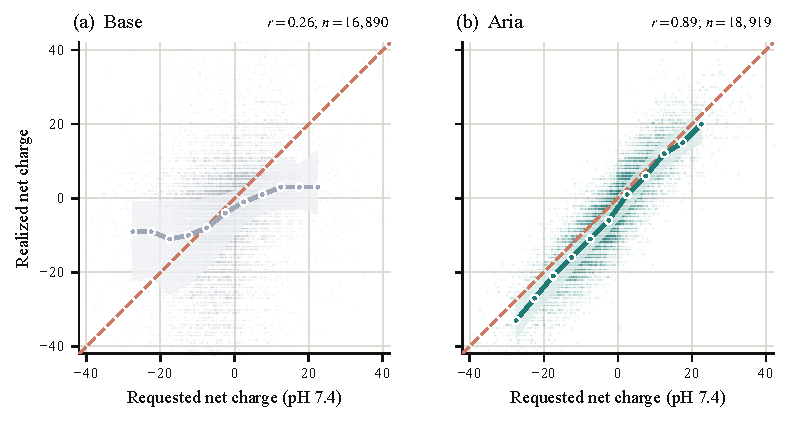
\includegraphics[width=0.9\linewidth]{figures/fig-charge-control-faceted.pdf}
\caption{Requested versus realized net charge at pH 7.4 for the base model
(a; $n=16{,}890$) and Aria (b; $n=18{,}919$). Faint points
represent individual valid generations; integer-valued requests are jittered
horizontally for visualization only. Solid lines show the median realized
charge within requested-charge bins, and shaded bands show the corresponding
interquartile ranges. The dashed line denotes exact agreement ($y=x$).
Pearson correlations are calculated using all valid charge-requesting outputs,
including observations outside the displayed range.}
\label{fig:charge}
\end{figure}


\section{Domain adherence against significance}\label{app:domain}
$N = 17{,}941$ fine-tuned generations whose specification requested a domain. The last row is \texttt{hmmscan}'s default reporting threshold with no further
filtering, and is the 2.90\pct{} quoted in the text. The baseline records 0
successes in 15{,}140 generations at every threshold.
\begin{table}[h]
\caption{Pfam-domain recovery across hmmscan reporting thresholds. 
Lower $E$-values indicate stronger
sequence-profile matches. Stricter thresholds reduce coverage but substantially
increase the specificity of the retained assignments.\\}
\label{tab:domain-thresholds}
\centering
\small
\begin{tabular}{lrrr}
\toprule
$E$-value & Any significant assignment & Requested domain
& $P(\text{correct}\mid\text{any})$ \\
\midrule
$10^{-10}$ & 145 \enspace(0.8\pct)      & 0.57\pct & 71.0\pct \\
$10^{-5}$  & 380 \enspace(2.1\pct)      & 1.38\pct & 65.3\pct \\
$10^{-3}$  & 649 \enspace(3.6\pct)      & 1.95\pct & 53.9\pct \\
$10^{-2}$  & 1{,}206 (6.7\pct)          & 2.23\pct & 33.2\pct \\
$10^{-1}$  & 4{,}173 (23.3\pct)         & 2.60\pct & 11.2\pct \\
$10^{1}$ (default) & 7{,}607 (42.4\pct) & 2.90\pct & 6.8\pct \\
\bottomrule
\end{tabular}
\end{table}
\begin{figure}[t]
\centering
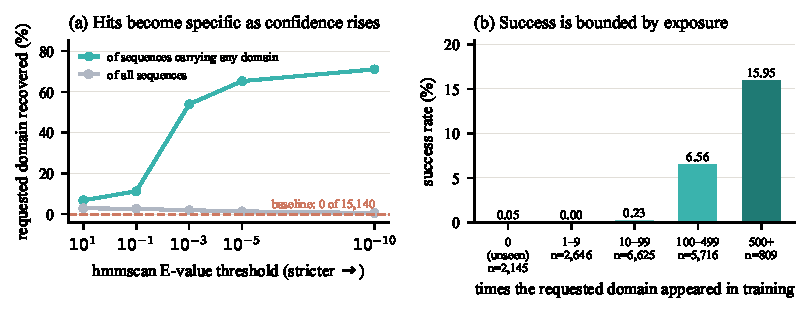
\includegraphics[width=\linewidth]{figures/fig3-domain.pdf}
\caption{Domain adherence is rare, targeted, and bounded by exposure.
(a) As the hmmscan threshold tightens, fewer generations carry
any significant assignment but the probability such an assignment is the
requested one rises to 71\pct; the baseline records zero successes at every
threshold. (b) Attempt-weighted success against how often the requested
domain appeared in training.}
\label{fig:domain}
\end{figure}

\section{Enzyme-class adherence is confounded by the predictor}\label{app:ec}
Across the 32 EC classes requested at least 50 times, the correlation between
how frequently CLEAN emits a class over the whole evaluation and that class's
apparent success rate is $r = 0.96$; the value is stable between 0.90 and 0.96
for every class-size cutoff we tried. EC~7.4 was requested 129 times and never
predicted for any sequence, so its zero was guaranteed by the predictor;
EC~1.2 was requested 609 times and predicted three times. Conversely EC~3.2 was
predicted roughly fourteen times more often than requested and shows 46.6\pct{}
apparent success. We therefore exclude enzyme class from the reported adherence results, and report the diagnostic rather than the number.

\section{The constraint ladder}\label{app:ladder}
\begin{table}[b]
\caption{Length adherence across the nested constraint ladder. Each rung adds
the listed descriptor to the preceding specification while retaining the same
length target ($n=200$ cluster-separated held-out proteins per rung and model;
one generation per prompt). Values are the percentages of generations within
$\pm10\pct{}$ of the requested length.}
\label{tab:ladder}
\centering
\small
\begin{tabular}{rlrr}
\toprule
Descriptors & Added at this rung & Aria & Base \\
\midrule
1  & (length target only)  & 90.0\pct & 7.0\pct \\
2  & net charge            & 86.5\pct & 7.0\pct \\
3  & hydrophobicity        & 84.5\pct & 9.0\pct \\
4  & stability             & 86.5\pct & 9.5\pct \\
5  & aggregation           & 90.5\pct & 6.0\pct \\
6  & cysteine count        & 89.5\pct & 7.5\pct \\
7  & structural confidence & 90.5\pct & 14.0\pct \\
8  & transmembrane helix   & 92.0\pct & 10.0\pct \\
9  & signal peptide        & 92.0\pct & 9.0\pct \\
10 & Pfam domain           & 91.5\pct & 7.5\pct \\
11 & EC class              & 90.0\pct & 8.5\pct \\
12 & molecular function    & 90.5\pct & 8.5\pct \\
13 & organism              & 87.5\pct & 7.0\pct \\
\bottomrule
\end{tabular}
\end{table}

To isolate prompt load from target difficulty, we constructed a nested constraint ladder for each of 200 cluster-separated held-out proteins. For each, we build thirteen prompts.All thirteen prompts for a protein shared the same length target. The first requested length alone, and each subsequent prompt added one further descriptor, yielding zero to twelve additional properties. Each model generated one sequence per prompt, and length adherence was defined as falling within $\pm10\pct{}$ of the fixed target ($n=200$ per rung per model). Each
rung is 200 generations, 2{,}600 in total. Adherence stays between 84.5\pct{}
and 92.0\pct{} across the ladder. The base model stays
near its unconditioned rate throughout. This experiment is specific to preservation of the fixed length target; it does not establish that every conditioned property is equally insensitive to prompt load.

\section{Training footprint}\label{app:compute}
Stage 1 is 348{,}867 examples over 21{,}804 optimizer steps (two epochs) on two
A100-80GB GPUs, $\sim$35 GPU-hours total, updating 83.9M
parameters ($\sim$1\pct{} of the model). Stage 2 is 929 preference pairs over 60
steps on one GPU with $\beta = 0.5$ and $\alpha_{\text{RPO}} = 1.0$; its
optimizer cost is negligible beside its oracle cost of 19{,}904 sampled
candidates and ESMFold on the survivors.

\emph{Constraint score}, used by the Stage-2 gate at a floor of 0.70, is the
mean per-axis satisfaction over the sequence-verifiable axes a prompt states: 1
for a bin matched exactly, 1 for length within $\pm$10\pct{} and charge within
$\pm$2 degrading linearly to 0 at twice tolerance, likewise for an exact
cysteine count, and 0 for a sequence that is not a clean peptide. Axes needing
an external predictor are excluded by construction, so the score cannot reward
guessing at them.

Anchoring the preferred response on a natural sequence is what makes the update
safe. With both responses drawn from the model, the DPO objective depends only
on the \emph{difference} of the two log-ratios, so it can be reduced by pushing
the rejected response down which drags the preferred one with it. Diversity after
the anchored round does not contract: mean within-set pairwise identity is 0.440
against 0.557 for the natural held-out set, and identity to a consensus built
from the training sequences is 0.568 against 0.647.

Because the policy was supervised-trained on the same natural responses later used as preferred examples, memorization is a live concern. Mean identity to the nearest training sequence rises from 0.184 after supervised fine-tuning to 0.354, reaching 0.658 among the 19 generations that pass the full conjunction, and 2 of 255 outputs with an extractable sequence are at least 90\pct identical to a training sequence. A control on the natural family settles the interpretation: real held-out members of PF00416 sit at 0.707 mean identity to their nearest training protein, and 29 of 260 (11\pct) exceed 90\pct. The family is highly conserved, so genuine homologues are already this similar to one another. Generated sequences are therefore less similar to the training set than real proteins of the same family are, and cross the near-copy threshold an order of magnitude less often.

\section{Worked examples}\label{app:examples}
Two of the nineteen held-out uS13 specifications whose generations satisfied
the full conjunction are shown below. Realized values are recomputed from the generated
sequences with the functions used to construct their specifications.

\paragraph{B1MVZ2: 4 properties requested, all scorable ones met} (confidence 79.1).
Requested length 123 (realized 119, within $\pm10\pct{}$) and cysteine count 0
(0); aggregation low (low); organism \emph{Leuconostoc citreum} (strain KM20)
was conditioned on but not scored.

\medskip
\noindent\textbf{Generated sequence:}
\begin{small}
\begin{verbatim}
MARIAGVNIPTNKRVVIALQYIHGIGTKFAQEILEKVGIPAERRVNQLTDAEVLQIRETI
DRDYQVEGDLRRETSMNIKRLMDLGSYRGLRHRRGLPVRGQRTKTNARTRKGPRKPIKK
\end{verbatim}
\end{small}

\paragraph{B8I805: 8 properties requested, all scorable ones met} (confidence 78.2).
Requested length 122 (realized 121), hydrophobicity low (low), stability stable
(stable), aggregation low (low), and cysteine count 1 (1); structural
confidence high, domain PF00416, and molecular function rRNA binding were
conditioned on but not scored.

\medskip
\noindent\textbf{Generated sequence:}
\begin{small}
\begin{verbatim}
MARIAGVNIPTNKRVEIALTYIHGIGRFVAGQIIEKVGIPAERRVNQLTDADIDKLREEV
GKFIVEGDLRREVAMNVKRLMDLGCYRGLRHRRGLPVRGQRTKTNARTRKGPRKTVAGKKK
\end{verbatim}
\end{small}

\begin{figure}[H]
\centering
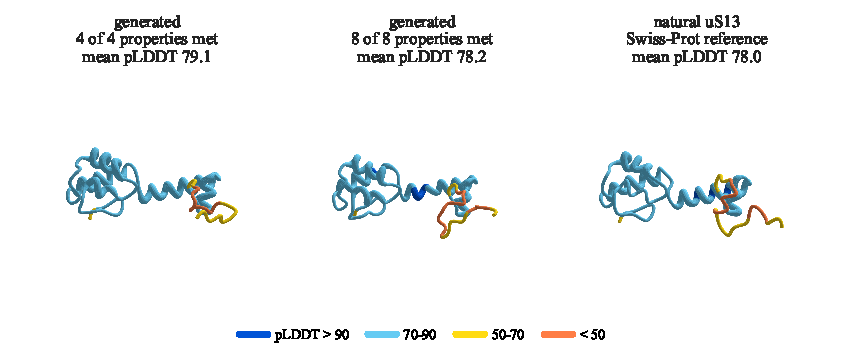
\includegraphics[width=\linewidth]{figures/fig-examples.pdf}
\caption{Predicted structures for the two generations described above, beside
a natural uS13 sequence from the same family. Spline-smoothed
$\mathrm{C}\alpha$ tubes are thickened through helices and strands and colored
by per-residue ESMFold confidence; all three structures are shown along their
principal axes under identical lighting.}
\label{fig:examples}
\end{figure}

\end{document}